\section{Phase 2: Low Fidelity Prototype}
We used the results from our preliminary survey to inform our initial design work. Our focus on AR allowed us to explore how critical factors of online experiences identified in the original survey, such as access to reviews, could be brought into the store environment while preserving aspects of in-store decision making, such as being ``hands-on with the product'' and leaving the store with the product. \todo{DNS: Is there a quote that can go here? MW: This is a quote from our early survey. Is it worth including/does it need to be cited? I could also dig something up from a related paper.}

\begin{marginfigure}
	\begin{minipage}{\marginparwidth}
			\centering
			\subfloat[][Context-aware paper prototype]{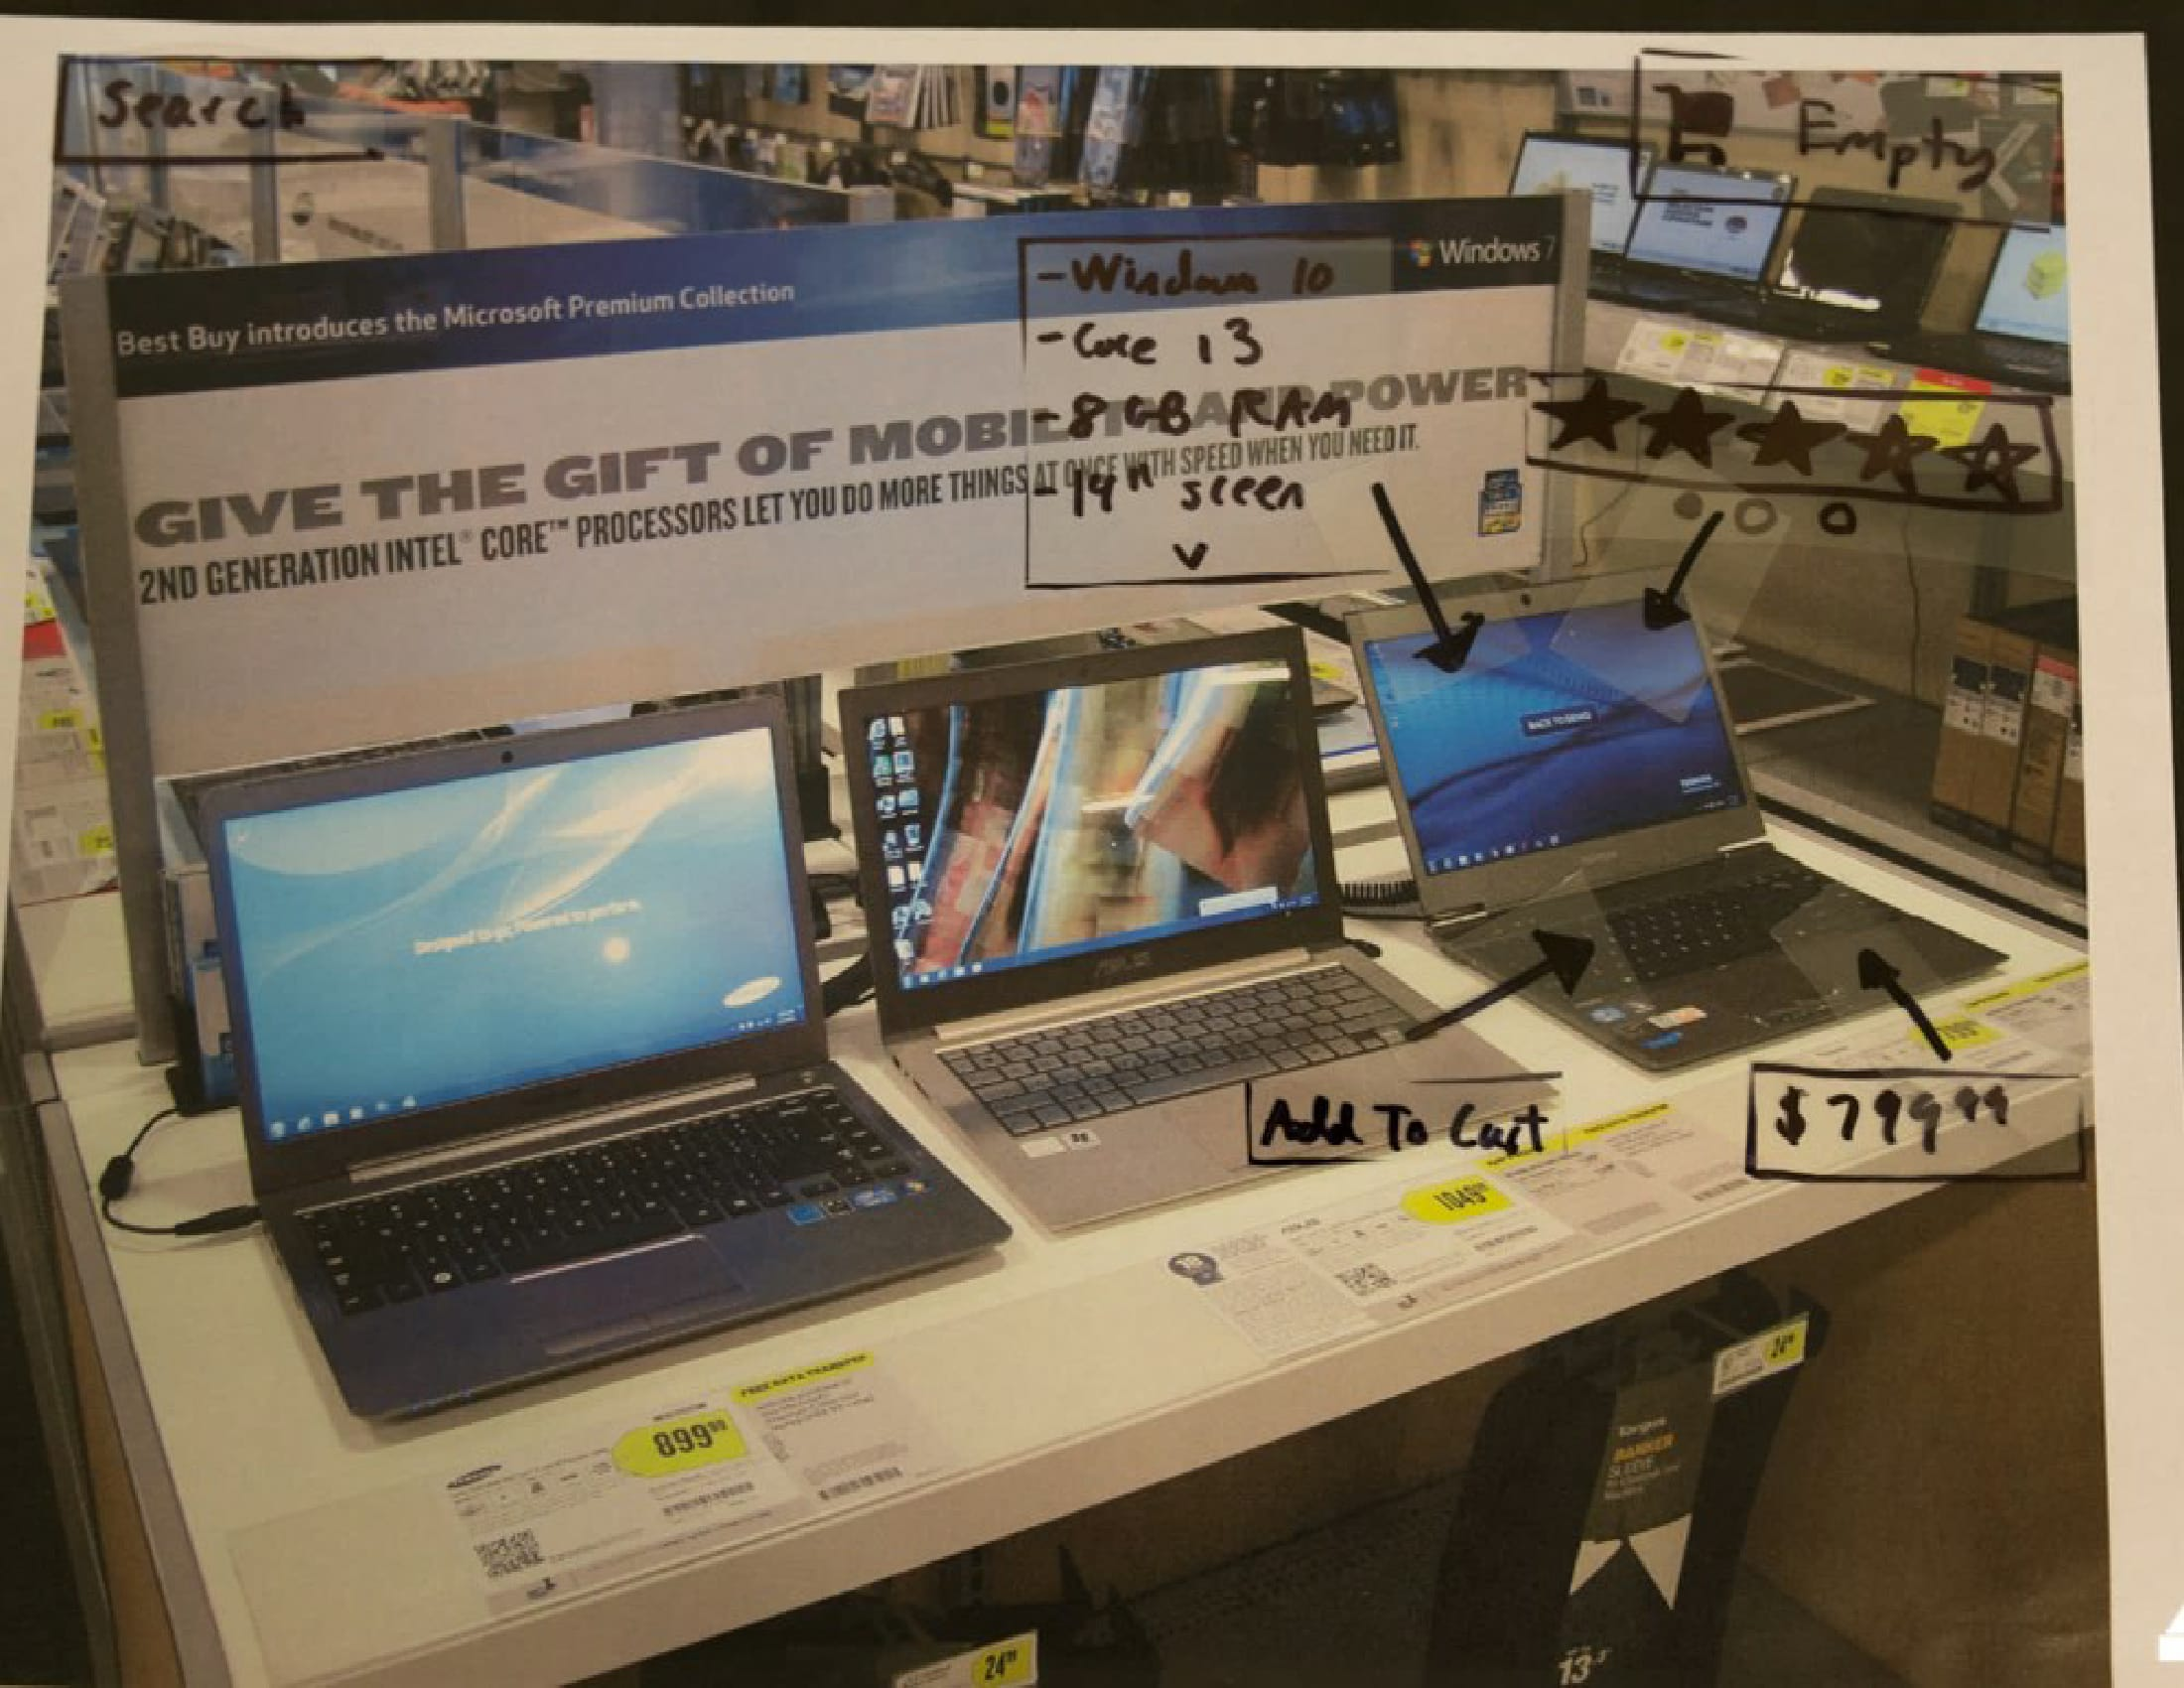
\includegraphics[width=0.9\columnwidth]{figures/LowFiContext}~\label{fig:LowFiContext}}
			\vfill
			\subfloat[][Menu-based paper prototype]{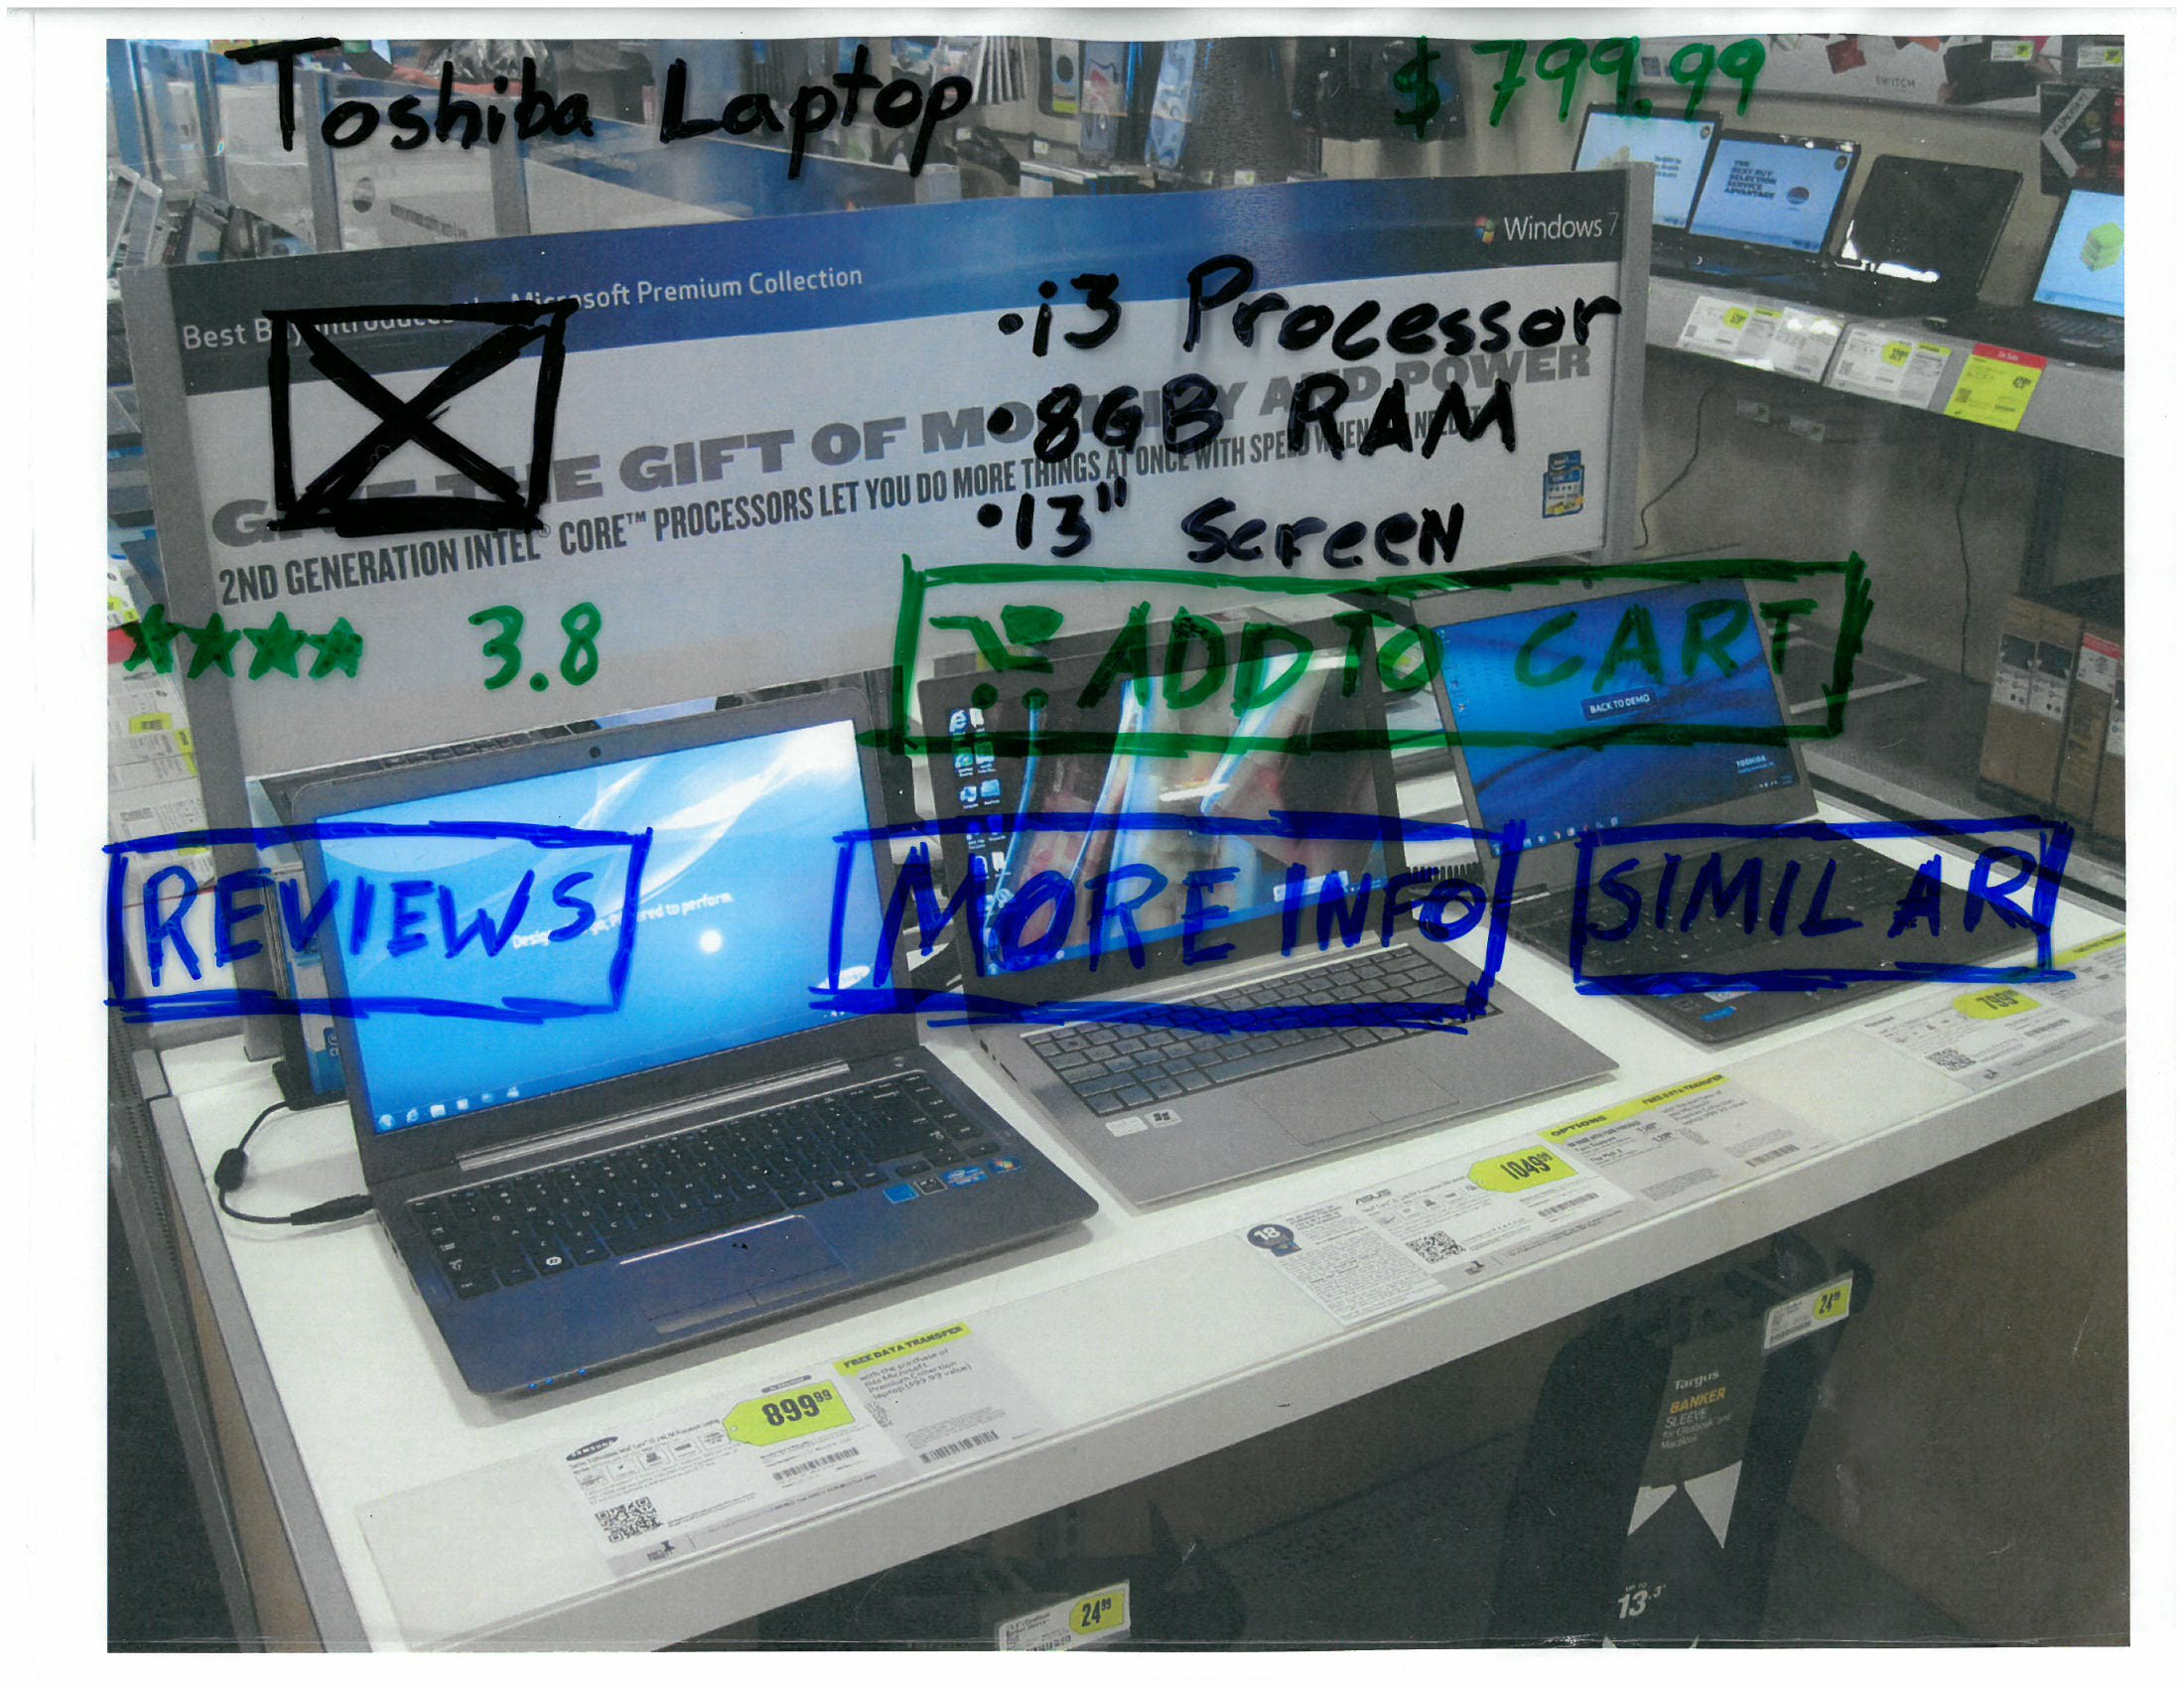
\includegraphics[width=0.9\columnwidth]{figures/LowFiMenu}~\label{fig:LowFiMenu}}
		\caption{Phase Two compared perceptions of a context-based and menu-based approach to augmenting traditional retail shopping with important factors of online shopping identified by participants in Phase One. }
	\end{minipage}
\end{marginfigure}

We hypothesized that an augmented reality application that supplemented a traditional in-store experience with immediate access to core aspects of online shopping would improve consumer's confidence in their purchasing decisions. \todo{replace the last bit of this sentence with what was actually tested} \todo{JRB: This sentence needs to be integrated once the correct content is put in there.} We used the results from our survey to design two sketch-based low fidelity prototypes of an AR system containing aspects of in-store and online shopping experiences that survey participants from Phase One identified as important. The prototypes, shown in Figures \ref{fig:LowFiContext} and \ref{fig:LowFiMenu}, consisted of online content drawn as AR menus on transparency sheets and overlaid onto an image of an electronics store. 
We used the two prototypes to make a comparison between hierarchical menu-based content and context-aware virtual overlays of price, review and specification information. We collected feedback on our designs through a think-aloud with three participants.
% study using our sketch-based prototypes as a design prompt. \todo{JRB: Formative design work and evaluation do not have to be hypothesis driven, and often aren't. Instead they are exploratory. If you are feeling encumbered by the "hypothesis" language, we can reword. Just let me know.} 

Participants were asked to choose which laptop they would purchase for each condition, with system type randomly ordered.  \todo[inline]{what specific AR components were tested here (e.g., reviews, product comparisons, specs, etc.)? What were your measures here (e.g., confidence in the decision, time to decision, etc.) MW: Briefly explained that in previous sentence} \todo{JRB: How did you analyze the data from this phase? MW: In English: We listened to them talk out loud and they told us how they are using the system in decision-making.} We recorded user feedback as participants navigated the two systems. Our focus was on qualitative responses informing us how this system helped them make a purchase decision.

Generally, participants were more receptive to quick and less information than to the fuller, menu-based approach. The non-obstructive nature and location-sensitive, quick information, and fewer interactions required provided by the context-aware prototype allowed for faster decision-making and increased understanding of the system's capabilities. \todo{JRB: Why? DNS--And how does this fit in with the design for Phase Three? MW: Basically, they weren't confused and did things faster} Participants specifically mentioned the ability to compare the specifications of two different laptops in the same view, the ability to toggle display of content, and visual product demonstrations as a useful features for increased efficiency and more empowered decision-making.

Our findings from the first two phases informed how we would approach the third phase of the design process. For the final prototype, we derived content from the early survey, empowering the user with important aspects of the virtual experience without sacrificing key aspects of the physical one. Considering the feedback from this prototyping phase, we took a context-aware approach to content delivery in the final phase of the design process. \todo{JRB: This is a list of what they told you. Can you take it one step further and tell us what this means? What are the implications of these comments? You said you did this -- "We explored how understanding the trade-offs of parallel physical and virtual experiences could inform mixed reality applications in the context of retail shopping." -- so tell me what the results of this phase told you about those trade-offs. MW: I think this is what you had in mind}
